%%%%%%%%%%%%%%%%%%%%%%%%%%%%%%%%%%%%%%%%%%%%%%%%%%%%%%%%%%%%%%%%%%%%%%%%%%%%%%%%
%% MASTER'S THESIS                                                            %%
%%                                                                            %% 
%% Title (en): Mining Parallel Corpora from the Web                           %%
%% Title (sk): Rafinácia paralelných korpusov z webu                          %%
%%                                                                            %%
%% Author: Bc. Jakub Kúdela                                                   %%
%% Supervisor: Doc. RNDr. Irena Holubová, Ph.D.                               %%
%% Consultant: RNDr. Ondřej Bojar, Ph.D.                                      %%
%%                                                                            %%
%% Academic year: 2015/2016                                                   %%
%%%%%%%%%%%%%%%%%%%%%%%%%%%%%%%%%%%%%%%%%%%%%%%%%%%%%%%%%%%%%%%%%%%%%%%%%%%%%%%%

\chapter{Web Data (Common Crawl) Experiment}
\label{chapter:web_data_common_crawl_experiment}

In this chapter, the second experiment conducted with our method is discussed. Unlike the first experiment (see Chapter~\ref{chapter:prealigned_data_czeng_experiment}) this one deals with the non-parallel, real-word, noisy data acquired from the web. It illustrates effectiveness of our method in a typical situation for which it is designed.

The selected language pair is the same as in the first experiment, i.e.\ Czech--English. This experiment's procedure utilizes the training artifacts created in the first experiment, namely the dictionary, bilingual word vectors and the trained classifier. The input data are obtained from the July 2015 dataset provided by the Common Crawl organization (see Section~\ref{section:common_crawl}).

The following text describes the procedure of the experiment with an example approach to the task of mining parallel corpus from the Common Crawl dataset for a specific language pair. It also discusses the manually evaluated quality of the acquired Czech--English parallel corpus.

\section{Experiment Procedure}
\label{section:common_crawl_experiment_procedure}

The July 2015 dataset consists of approximately $1.84$ billions of crawled web pages and it takes about $149$ terabytes (TB) of disk space in the uncompressed WARC format. To process this large volume of data we use Hadoop (see Section~\ref{section:hadoop}) cluster provided by MetaCentrum (see Section~\ref{section:metacentrum}). The dataset is available in a form of $33,957$ WARC files compressed by GNU zip (gzip)\footnote{\url{http://www.gzip.org/} (accessed April 23, 2016)}. Each of these files has less than $950$ megabytes (MB) and is accessible via its own URL. The list of these URLs can be obtained at the official website of the Common Crawl~\cite{CommonCrawl} organization. The total size of the July 2015 dataset in the compressed format is approximately $28.5$ TB.

One of the options to get all the files into HDFS (see Subsection~\ref{subsection:hdfs}), is to download them in sequence with cURL\footnote{\url{https://curl.haxx.se/} (accessed April 23, 2016)} using one node of the cluster. During the process, every downloaded file can be immediately copied into HDFS using the command \texttt{hadoop fs -copyFromLocal} and afterwards deleted locally. To reduce the time, the process can use multiple threads. In our environment, we use $5$ threads and the described process takes about $17$ days to complete. Such a long process can be interrupted by many circumstances (e.g.\ cluster maintenance). Therefore, our script first checks which of the files are already present in HDFS using the command \texttt{hadoop fs -ls} to avoid repetitive downloading. Hadoop allows the user to process the WARC files compressed by gzip. We use this feature to reduce the required disk space at the cost of slower execution.

\begin{figure}[!htb]
	\centering
	\caption{Common Crawl experiment}
	\label{figure:common_crawl_experiment}
	\vspace{1em}
	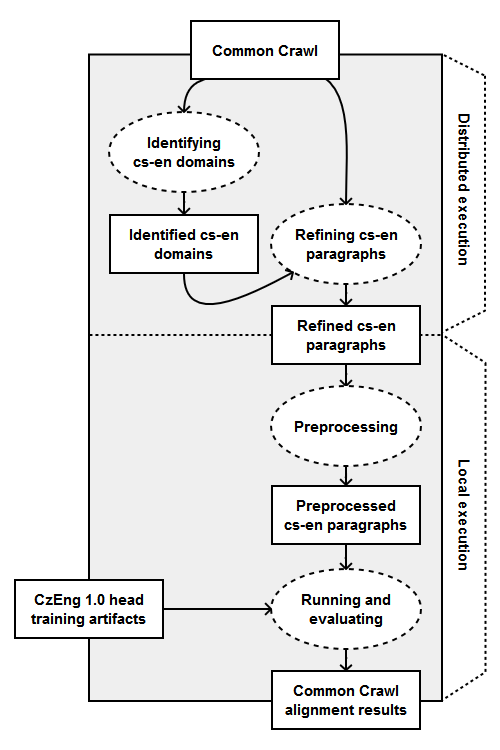
\includegraphics[width=0.65\textwidth]{images/common_crawl_experiment.png}
\end{figure}

With the entire July 2015 dataset stored in HDFS, the experiment illustrated in Figure~\ref{figure:common_crawl_experiment} is applied. The procedure starts with the distributed execution running two MapReduce (see Subsection~\ref{subsection:mapreduce}) jobs. This creates a dataset containing Czech and English paragraphs from the web domains identified to be bilingual. The paragraphs are then aligned with our method in a local execution and the results are evaluated. The whole process is described as follows.

\subsection{Distributed Execution}
\label{subsection:common_crawl_distributed_execution}

The part of the experiment's procedure executed in the distributed environment consists of two MapReduce jobs. The first job identifies the web domains containing paragraphs in both the languages we are interested in. In order to enable the MapReduce framework to read and write the WARC files properly we use WARC-Hadoop (See Section~\ref{section:warc_hadoop}).

Let us describe the implementations of the mapper and the reducer in the first MapReduce job. The mapper is called \textit{WarcTextMapper}. It iterates through the WARC records processing only those which represent HTTP responses with \texttt{text/html} content type, i.e.\ web pages. For every web page it resolves the character encoding and transforms its HTML structure into XHTML using jsoup (see Section~\ref{section:jsoup}). Then, the textual contents of all the \texttt{<p>} HTML tags representing paragraphs are parsed and all those having less than $100$ characters are discarded. The shorter paragraphs are discarded because it is difficult to detect their language reliably. For each paragraph the language is identified with a certain confidence using language-detector (see Section~\ref{section:language_detector}) . The mapper outputs a key-value pair for each paragraph where the language is detected as one of the two languages we are interested in with the confidence at least $99\%$. The structure of an output key-value pair is following:

\vbox{
\begin{itemize}
	\item Key: web domain name.
	\item Value: 
	\begin{enumerate}[label=$\circ$]
		\item language detected by language-detector;
		\item confidence returned by language-detector;
		\item URL associated with the paragraph;
		\item textual content of the paragraph.
	\end{enumerate}
\end{itemize}
}
	
The implementation of the reducer is called \textit{WarcDomainReducer}. For a given web domain (i.e.\ key) it receives the values representing all the paragraphs for the domain emitted by \textit{WarcTextMapper}. The reducer iterates over all these values counting the number of the unique paragraphs (using hashing) and their total length for both the languages separately. It also counts the number of the unique URLs. For every domain having at least one Czech and one English paragraph the reducer outputs the key-value pair as follows:

\vbox{
\begin{itemize}
	\item Key: web domain name.
	\item Value: 
	\begin{itemize}[label=$\circ$]
		\item number of unique URLs;
		\item number of unique English paragraphs;
		\item total length of unique English paragraphs;
		\item number of unique Czech paragraphs;
		\item total length of unique Czech paragraphs.
	\end{itemize}
\end{itemize}
}

The first MapReduce job creates a list of web domains having at least some Czech and English content. Listing~\ref{listing:experiment_domains} shows a sample from its output file. The format contains tab-separated values, where the first column is a web domain, which is the key. The other columns represent the individual items of the value in the order they were listed. The list contains $12,144$ domains. 

\begin{lstlisting}[float=!htb,caption={sample from a file with identified domains},label={listing:experiment_domains},firstnumber=3874]
www.meuslany.cz		2	6	2813	16	4509
www.mff.cuni.cz		7	37	14946	39	18162
\end{lstlisting}

As the next step, a filter is applied on the output of the first MapReduce job reducing the number of web domains to be considered for the further processing. The filter requires from a domain to meet the following condition:
	
\begin{align*}
\frac{\min(N_{cs},N_{en})}{\max(N_{cs},N_{en})} > 1\%,
\end{align*}
	
where $N_{cs}$ and $N_{en}$ are the numbers of Czech and English paragraphs for the domain respectively. The filtering discards all the domains having very unbalanced language distribution. The output contains $8,750$ identified bilingual domains.

The second MapReduce job extracts the Czech and English paragraphs for all the identified bilingual web domains. It uses the same mapper as the first job; however, the implementation of the reducer is different. We call it \textit{WarcTextReducer}. In order to provide the reducer with the file containing the domains Hadoop Distributed Cache is utilized. It is a facility provided by the MapReduce framework enabling the user to cache files for a MapReduce job. Once a file is cached for a job the framework makes it available locally at each node of the cluster for the time of the execution allowing mappers and reducers to read the cached file. When initializing, \textit{WarcTextReducer} reads the entire file with the bilingual domains creating a set of hash codes for all their names. When running, it outputs only those incoming key-value pairs emitted by \textit{WarcTextMapper} that are associated with one of the domains. Additionally, all the values representing duplicate paragraphs are discarded. The structure of the output key-value pairs emitted by both \textit{WarcTextMapper} and \textit{WarcTextReducer} is identical.

Listing~\ref{listing:experiment_paragraphs_cs} and Listing~\ref{listing:experiment_paragraphs_en} show samples of two lines from the output file of the second MapReduce job. These two lines contain parallel paragraphs that are mutual translations. The single output file contains the paragraphs for both the languages. The format is a list of tab-separated values. The first column is a web domain, which is the key. The following columns represent the individual items of the value in the order they were listed in the text describing the structure of the output key-value pairs emitted by \textit{WarcTextMapper}. The output file contains $5,931,091$ paragraphs for both the languages, namely $801,116$ Czech and $5,129,975$ English. The Czech and English paragraphs originate from $127,570$ and $744,074$ unique URLs, respectively. The average length of a Czech paragraph is $352.78$ characters, while for an English one, it is $417.03$.

\begin{lstlisting}[float=!htb,caption={sample from a file with extracted paragraphs (Czech)},label={listing:experiment_paragraphs_cs},firstnumber=3185636]
czechfolks.com	cs	0.99999445885996	http://czechfolks.com/2009/11/25/how-well-do-you-know-the-czech-republic-sweepstakes-results-jak-dobre-znate-ceskou-republiku-a-vysledky-souteze/	Zde je otázka, kterou jsme položili a její správná odpověď: Otázka: Kdo byl Karel IV? Odpověď: Český král a římský císař.
\end{lstlisting}

\begin{lstlisting}[float=!htb,caption={sample from a file with extracted paragraphs (English)},label={listing:experiment_paragraphs_en},firstnumber=3185639]
czechfolks.com	en	0.9999980969126909	http://czechfolks.com/2009/11/25/how-well-do-you-know-the-czech-republic-sweepstakes-results-jak-dobre-znate-ceskou-republiku-a-vysledky-souteze/	Here is the question that we asked with the correct answer: Question: Who was Charles IV? Answer: The king of Bohemia and Holy Roman Emperor.
\end{lstlisting}

\subsection{Local Execution}
\label{subsection:common_crawl_local_execution}

The file containing the extracted paragraphs is transferred from HDFS to a one node of the cluster. The process continues in a single-node execution. The input dataset for our method is formed by distributing the paragraphs into the bins according to domain names. For each bilingual web domain, a bin is created with all the associated paragraphs in both the languages. This restricts the method to align only the paragraphs belonging to the same domain.

The rest of the procedure is similar as for the tail in the first experiment with CzEng 1.0 (see Section~\ref{subsection:czeng_experiment_running}). The input dataset is preprocessed by tokenization and lowercasing and our method is executed creating refined alignments for the paragraphs. The method is provided with the training artifacts created during the first experiment using the head of CzEng 1.0, namely the dictionary, bilingual word vectors and the trained classifier. The only difference in the settings is the changed confidence threshold for the classifier, which is required to be $99\%$. The precision is favoured over the recall. 

It is important to note that for this experiment the Czech language is selected as the source language. Therefore, the paragraph vectors associated with the English language are the ones indexed by Annoy. This selection follows the already mentioned rule of thumb (see Section~\ref{section:method_discussion}) to let the method index the document vectors for the language having more documents.

\section{Experiment Results}
\label{section:common_crawl_experiment_results}

Table~\ref{table:common_crawl_domains} lists the most frequent web domains appearing in the extracted pairs of paragraphs. The full list contains $2,178$ domains having altogether $114,711$ pairs of aligned paragraphs. This means, that the output of our method contains an alignment for $14,32\%$ of all the extracted Czech paragraphs. The extracted paragraph-aligned parallel corpus contains in total $7,235,908$ Czech and $8,369,870$ English tokens.

\begin{table}[!htb]
	\centering
	\caption{Common Crawl experiment: web domains of paragraph pairs}
	\label{table:common_crawl_domains}
	\vspace{1em}
	\begin{tabular}{|l|r|r|}
		\hline
		\textbf{Source Domain} & \textbf{Paragraph Pairs} & \textbf{Ratio (\%)} \\
		\hline
		europa.eu & 23457 & 20.45 \\
		eur-lex.europa.eu & 15037 & 13.11 \\
		windows.microsoft.com & 11905 & 10.38 \\
		www.europarl.europa.eu & 8560 & 7.46 \\
		www.project-syndicate.org & 2210 & 1.93 \\
		www.debian.org & 2191 & 1.91 \\
		support.office.com & 1908 & 1.66 \\
		www.esa.int & 1308 & 1.14 \\
		www.eea.europa.eu & 1299 & 1.13 \\
		www.muni.cz & 1206 & 1.05 \\
		\vdots & \vdots & \vdots  \\
		\hline
		\textbf{Total} & 114,711 & 100.00 \\
		\hline
	\end{tabular}
\end{table}

The quality of the extracted corpus is evaluated manually on a set of randomly selected $500$ paragraph pairs. The inspected pairs are divided into few categories. The results of this subjective evaluation are displayed in Table~\ref{table:common_crawl_refine}. The pair of paragraphs is considered to be a human translation if it seems like created by a human. These are the most favorable ones. If the translation of the pair seems cumbersome, it is labeled as a product of machine translation. The partial match represents a situation when a paragraph is a translation of only a part of the other having some extra content. Everything else is labeled as a mismatch.

\begin{table}[!htb]
	\centering
	\caption{Common Crawl experiment: evaluation (500 paragraph pairs)}
	\label{table:common_crawl_refine}
	\vspace{1em}
	\begin{tabular}{|l|r|r|}
		\hline
		\textbf{Category} & \textbf{Count} & \textbf{Ratio (\%)} \\
		\hline
		Human translation & 466 & 93.20 \\
		Machine translation & 7 & 1.40 \\
		Partial match & 13 & 2.60 \\
		Mismatch & 14 & 2.80 \\
		\hline
		\textbf{Total} & 500 & 100.00 \\
		\hline
	\end{tabular}
\end{table}

To estimate the precision of our method, let us consider the pairs of paragraphs belonging to the categories of human and machine translation as the true positives. This way all the other pairs are regarded as the false positives. Table~\ref{table:common_crawl_precision} shows how the precision of the method changes with respect to the confidence threshold of the classifier.

\begin{table}[!htb]
	\centering
	\caption{Common Crawl experiment: precision (500 paragraph pairs)}
	\label{table:common_crawl_precision}
	\vspace{1em}
	\begin{tabular}{|r|r|r|r|}
		\hline
		\textbf{Conf.(\%)} & \textbf{True Pos.} & \textbf{False Pos.} & \textbf{Precision (\%)} \\ \hline
		99.00 & 473 & 27 & 94.60 \\
		99.10 & 464 & 25 & 94.89 \\
		99.20 & 456 & 23 & 95.20 \\
		99.30 & 446 & 20 & 95.71 \\
		99.40 & 435 & 17 & 96.24 \\
		99.50 & 415 & 16 & 96.29 \\
		99.60 & 404 & 16 & 96.19 \\
		99.70 & 386 & 12 & 96.98 \\
		99.80 & 357 & 7 & 98.08 \\
		99.90 & 286 & 3 & 98.96 \\
		\hline
	\end{tabular}
\end{table}

The task of estimating the recall of our method is more difficult. We would need to manually inspect all the paragraphs from every web domain selected for the evaluation. Therefore, let us perform the recall estimation for only one web domain with smaller number of paragraphs present in the input dataset. The selected web domain is \texttt{www.csa.cz}, the official website of Czech Airlines containing human-translated content. For the domain, the input dataset contains $68$ Czech and $87$ English paragraphs. These are manually aligned, creating what we consider to be the ideal alignments. When evaluated, the ideal alignments contain $44$ paragraph pairs, of which $42$ appear also in the corpus extracted by our method. Additionally, the corpus include $1$ extra pair subjectively regarded as mismatch. Table~\ref{table:common_crawl_effectiveness} shows the effectiveness of our method evaluated for the \texttt{www.csa.cz} web domain. The results are satisfactory; however, \texttt{www.csa.cz} is a website with a large proportion of the content provided in both the languages. This fact makes it one of the cleaner sources of parallel Czech--English content.

\begin{table}[!htb]
	\centering
	\caption{Common Crawl experiment: effectiveness (\texttt{www.csa.cz})}
	\label{table:common_crawl_effectiveness}
	\vspace{1em}
	\begin{tabular}{|l|r|}
		\hline
		\textbf{Recall (\%)} & 95.45 \\
		\hline
		\textbf{Precision (\%)} & 97.67 \\
		\hline
	\end{tabular}
	\vspace{2em} 
\end{table}

\section{Experiment Time Duration}
\label{section:common_crawl_experiment_duration}

The cluster used for the distributed execution of the MapReduce jobs is described in Section~\ref{section:metacentrum}. The rest of the procedure, i.e.\ the local execution, is done on one node of the cluster having Intel\textregistered{} Xeon\textregistered{} CPU E5-2630 v3 (20 MB Cache, 2.40 GHz) and 128 gigabytes (GB) of memory. Table~\ref{table:common_crawl_time_duration} contains the approximate time durations of the individual steps of the experiment.

\begin{table}[!htb]
	\centering
	\caption{Common Crawl experiment: time duration}
	\label{table:common_crawl_time_duration}
	\vspace{1em}
	\begin{tabular}{|l|r|}
		\hline
		\multicolumn{1}{|c|}{\textbf{Activity}} & \multicolumn{1}{c|}{\textbf{Duration (hh:mm)}} \\
		\hhline{|=|=|}
		\multicolumn{2}{|c|}{\textbf{MapReduce framework}} \\
		\hline
		Identifying cs-en domains & 11:58 \\
		Refining cs-en paragraphs & 11:38 \\
		\hline
		\multicolumn{2}{|c|}{\textbf{Local Execution}} \\
		\hline
		Tokenization and lowercasing & 00:09 \\
		Generating document vectors & 00:58 \\
		Aligning document vectors (Annoy) & 01:13 \\
		Scoring alignments & 03:42 \\
		Applying network classifier & 00:39 \\
		\hline
	\end{tabular}
\end{table}
